%%%%%%%%%%%%%%%%%%%%%%%%%%%%%%%%%%%%%%%%%
% Beamer Presentation
% LaTeX Template
% Version 1.0 (10/11/12)
%
% This template has been downloaded from:
% http://www.LaTeXTemplates.com
%
% License:
% CC BY-NC-SA 3.0 (http://creativecommons.org/licenses/by-nc-sa/3.0/)
%
%%%%%%%%%%%%%%%%%%%%%%%%%%%%%%%%%%%%%%%%%

%----------------------------------------------------------------------------------------
%	PACKAGES AND THEMES
%----------------------------------------------------------------------------------------

\documentclass{beamer}

\mode<presentation> {

% The Beamer class comes with a number of default slide themes
% which change the colors and layouts of slides. Below this is a list
% of all the themes, uncomment each in turn to see what they look like.

%\usetheme{default}
%\usetheme{AnnArbor}
\usetheme{Antibes}
%\usetheme{Bergen}
%\usetheme{Berkeley}
%\usetheme{Berlin}
%\usetheme{Boadilla}
%\usetheme{CambridgeUS}
%\usetheme{Copenhagen}
%\usetheme{Darmstadt}
%\usetheme{Dresden}
%\usetheme{Frankfurt}
%\usetheme{Goettingen}
%\usetheme{Hannover}
%\usetheme{Ilmenau}
%\usetheme{JuanLesPins}
%\usetheme{Luebeck}
%\usetheme{Madrid}
%\usetheme{Malmoe}
%\usetheme{Marburg}
%\usetheme{Montpellier}
%\usetheme{PaloAlto}
%\usetheme{Pittsburgh}
%\usetheme{Rochester}
%\usetheme{Singapore}
%\usetheme{Szeged}
%\usetheme{Warsaw}

% As well as themes, the Beamer class has a number of color themes
% for any slide theme. Uncomment each of these in turn to see how it
% changes the colors of your current slide theme.

%\usecolortheme{albatross}
%\usecolortheme{beaver}
%\usecolortheme{beetle}
%\usecolortheme{crane}
%\usecolortheme{dolphin}
%\usecolortheme{dove}
%\usecolortheme{fly}
%\usecolortheme{lily}
%\usecolortheme{orchid}
%\usecolortheme{rose}
%\usecolortheme{seagull}
\usecolortheme{seahorse}
%\usecolortheme{whale}
%\usecolortheme{wolverine}

%\setbeamertemplate{footline} % To remove the footer line in all slides uncomment this line
%\setbeamertemplate{footline}[page number] % To replace the footer line in all slides with a simple slide count uncomment this line

%\setbeamertemplate{navigation symbols}{} % To remove the navigation symbols from the bottom of all slides uncomment this line
}

\usepackage{graphicx} % Allows including images
\usepackage{booktabs} % Allows the use of \toprule, \midrule and \bottomrule in tables
\usepackage{amsmath}

%----------------------------------------------------------------------------------------
%	TITLE PAGE
%----------------------------------------------------------------------------------------

\title[Infospreading]{Simulation of Information Spreading in a Facebook Network} % The short title appears at the bottom of every slide, the full title is only on the title page

\author{U. Lustenberger, N. Wili, P. Z\"ochbauer} % Your name
\institute[ETHZ] % Your institution as it will appear on the bottom of every slide, may be shorthand to save space
{
Federal Institute of Technology Zurich \\ % Your institution for the title page
\medskip
\textit{} % Your email address
}
\date{\today} % Date, can be changed to a custom date

\begin{document}

\begin{frame}
\titlepage % Print the title page as the first slide
\end{frame}

\begin{frame}
\frametitle{Overview} % Table of contents slide, comment this block out to remove it
\tableofcontents % Throughout your presentation, if you choose to use \section{} and \subsection{} commands, these will automatically be printed on this slide as an overview of your presentation
\end{frame}

%----------------------------------------------------------------------------------------
%	PRESENTATION SLIDES
%----------------------------------------------------------------------------------------

%------------------------------------------------
\section{Introduction} % 
%------------------------------------------------

\subsection{Social Networks} % 

\begin{frame}
\frametitle{Social Networks}
Facebook, Twitter, Instagramm, Tumblr, Google+ ....

\end{frame}


\subsection{Fundamental Questions}

\begin{frame}
\frametitle{Fundamental Questions}
\begin{itemize}

\item Are there relevant differences in the time evolution of the homogeneous SIR-model and the agent-based model?
\vspace{1cm}
\item Are there individuals which are more important to the spreading of information (Influentials)? Can they be recognized in the sense of position and connectivity in the network?


\end{itemize}
\end{frame}

%------------------------------------------------
\section{The Model} % 
%------------------------------------------------


\subsection{Reaction Equations}

\begin{frame}
\frametitle{Reaction Equations}

In the SIR-model as well as in the Agent-based model, the following set of ``reaction equations'' was used\\(I: Ignorant, S: Spreader, R: Stifler):\\
\vspace{1cm}



\begin{align}
& I + S \xrightarrow{\lambda} 2 S \\
& S + R \xrightarrow{\alpha} 2 R \\
& S + S \xrightarrow{\alpha} S + R 
\end{align}


\end{frame}



\subsection{Homogeneous SIR Model}
\begin{frame}
\frametitle{Homogeneous SIR Model}
Mathematically this can be expressed as a set of differential equations:\\


\begin{align}
& \frac{\text{d}i(t)}{\text{d}t} = -\lambda \cdot s(t)i(t)\\
& \frac{\text{d}s(t)}{\text{d}t} = \lambda \cdot s(t)i(t) - \alpha \cdot s(t)[s(t)+r(t)]\\
&\frac{\text{d}r(t)}{\text{d}t} = \alpha \cdot s(t)[s(t)+r(t)]
\end{align}


\end{frame}


\subsection{Inhomogeneous Agent-Based Model}
\begin{frame}
\frametitle{Agent-Based Model}

Flowchart??

\end{frame}


%------------------------------------------------
\section{Simulation} % 
%------------------------------------------------
\subsection{Characteristics}
\begin{frame}
\frametitle{Characteristics}

\begin{itemize}

\item Real facebook network
\vspace{1cm}
\item 384 Induviduals



\end{itemize}

\end{frame}

\subsection{Visualization}
\begin{frame}
\begin{center}
\huge{Video}

inklusive plot Spreader, stifler etc?

\end{center}
\end{frame}

\subsection{Variables for Analysis}
\begin{frame}[fragile]
\frametitle{Cumulative Infections}

Tree  \hspace{2.55cm} Infectpath 

\begin{columns}[c]

\column{0.33\textwidth}
\begin{figure}
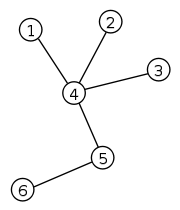
\includegraphics[scale=0.5]{tree}
\end{figure}

\column{0.33\textwidth}
\begin{tabular}{l r}
 6 & 5 \\
 5 & 4 \\
 4 & 1 \\
 4 & 2 \\
 4 & 3 \\
\end{tabular}

\column{0.3\textwidth}
\begin{verbatim}
cum_infections=
[0 0 0 3 4 5];
\end{verbatim}

\end{columns}
\end{frame}

%------------------------------------------------
\section{Results} % 
%------------------------------------------------

\subsection{Time Evolution}

\begin{frame}
\frametitle{Differences in Time Evolution}
\begin{center}
SIR-Model
\end{center}
\begin{center}
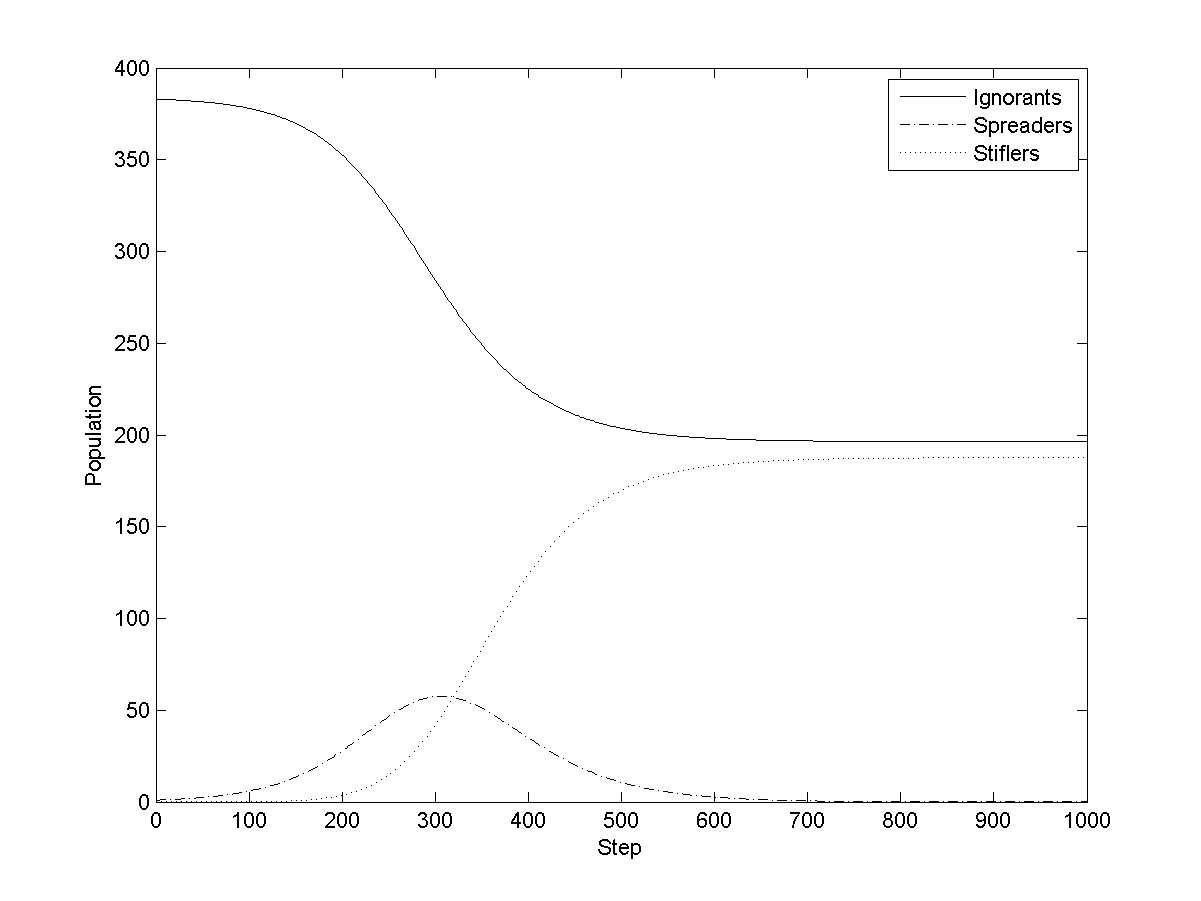
\includegraphics[width=9cm]{NICE_SIR}
\end{center}
\end{frame}

\begin{frame}
\begin{center}
Agent-based Model similar as SIR
\end{center}
\begin{center}
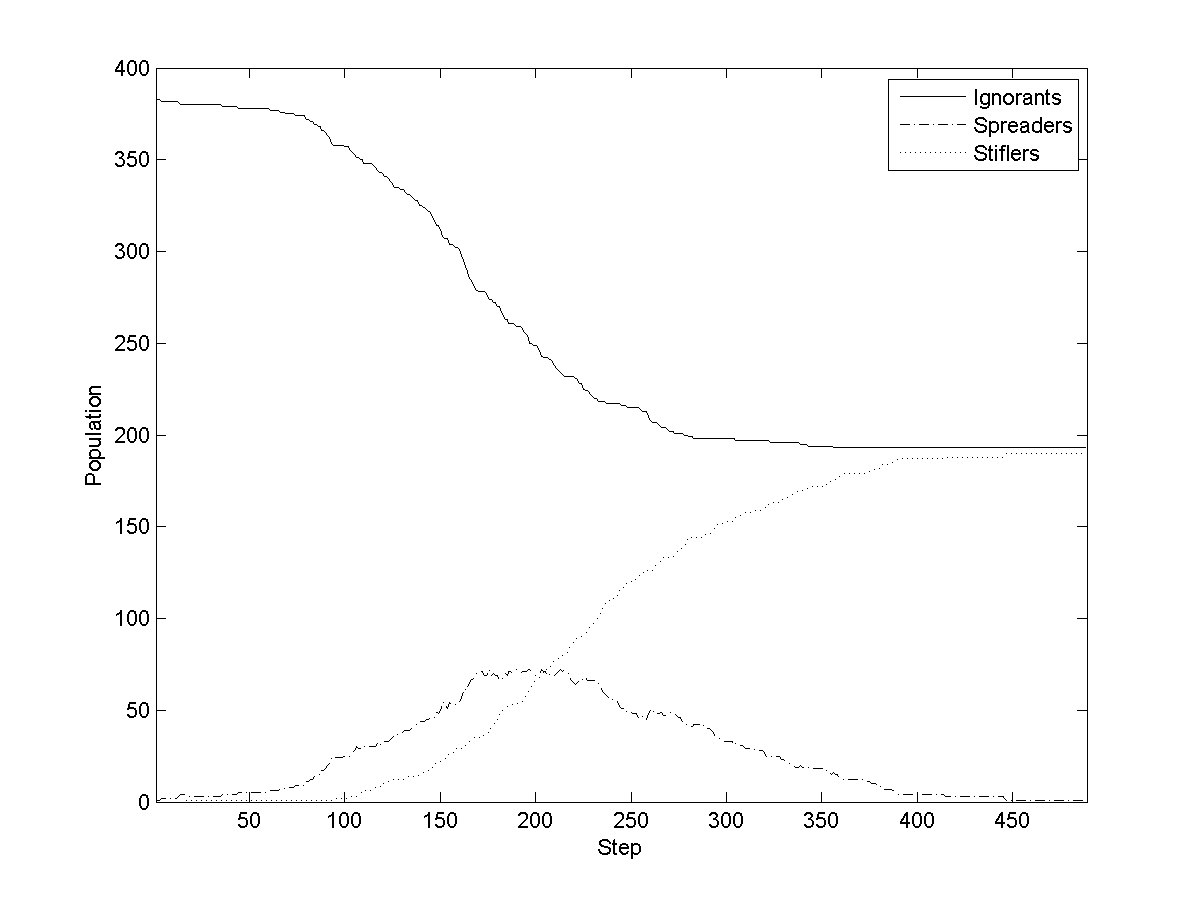
\includegraphics[width=9cm]{1-local-max}
\end{center}
\end{frame}

\begin{frame}
\begin{center}
Agent-based Model shows significant difference (two local max)
\end{center}
\begin{center}
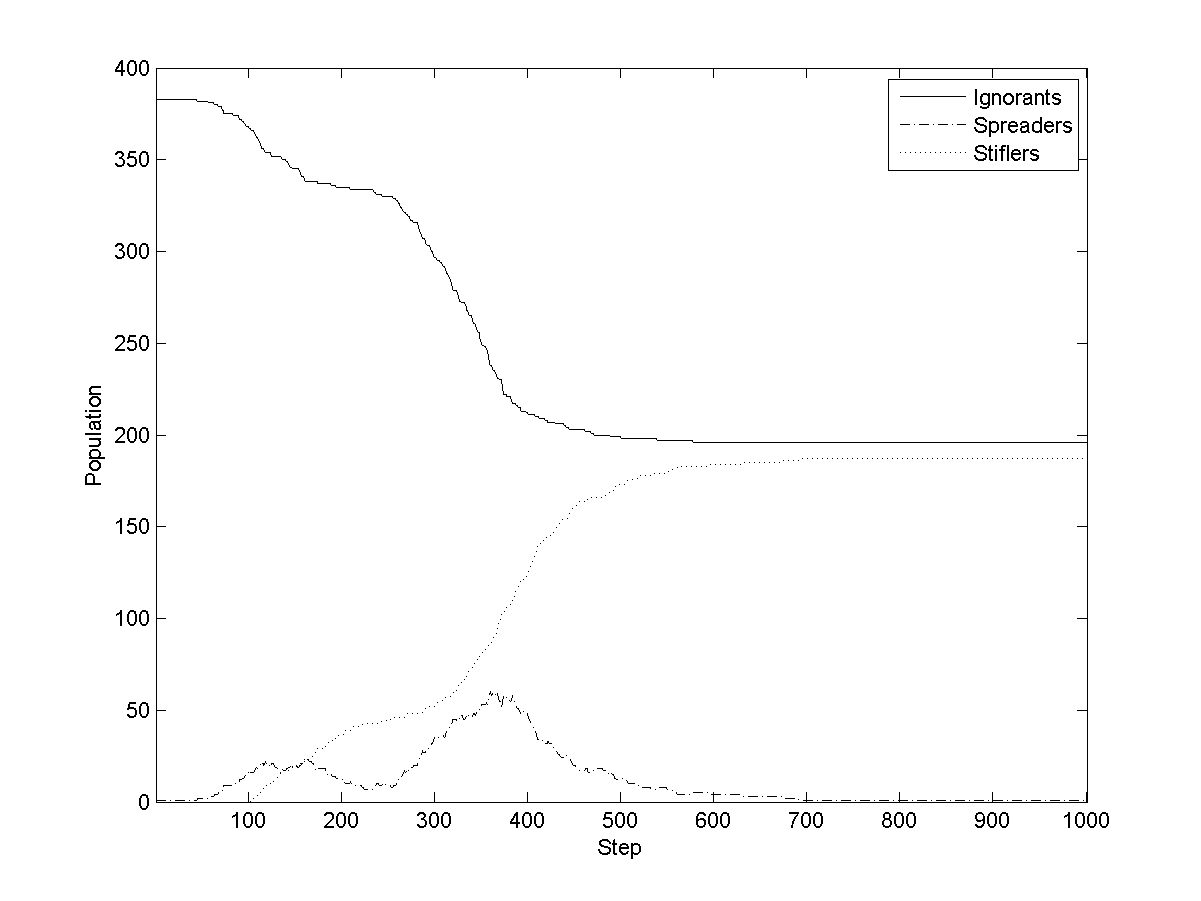
\includegraphics[width=9cm]{2-local-max}
\end{center}
\end{frame}

\subsection{Influentials}
\begin{frame}
\frametitle{Influentials}

Do influentials exist?

\begin{figure}
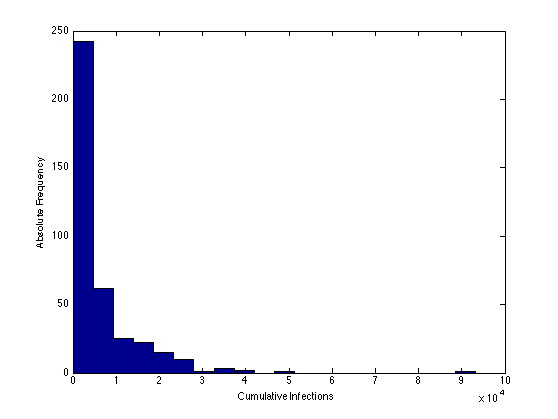
\includegraphics[width=7cm]{influ2}
\label{Histo}
\end{figure}


\end{frame}


\begin{frame}
\frametitle{Influentials}

Can we determine influentials from the characteristics of our network? (Clustercoefficient, Betweenness centrality)
\begin{columns}[c]

\column{0.48\textwidth}
\begin{figure}
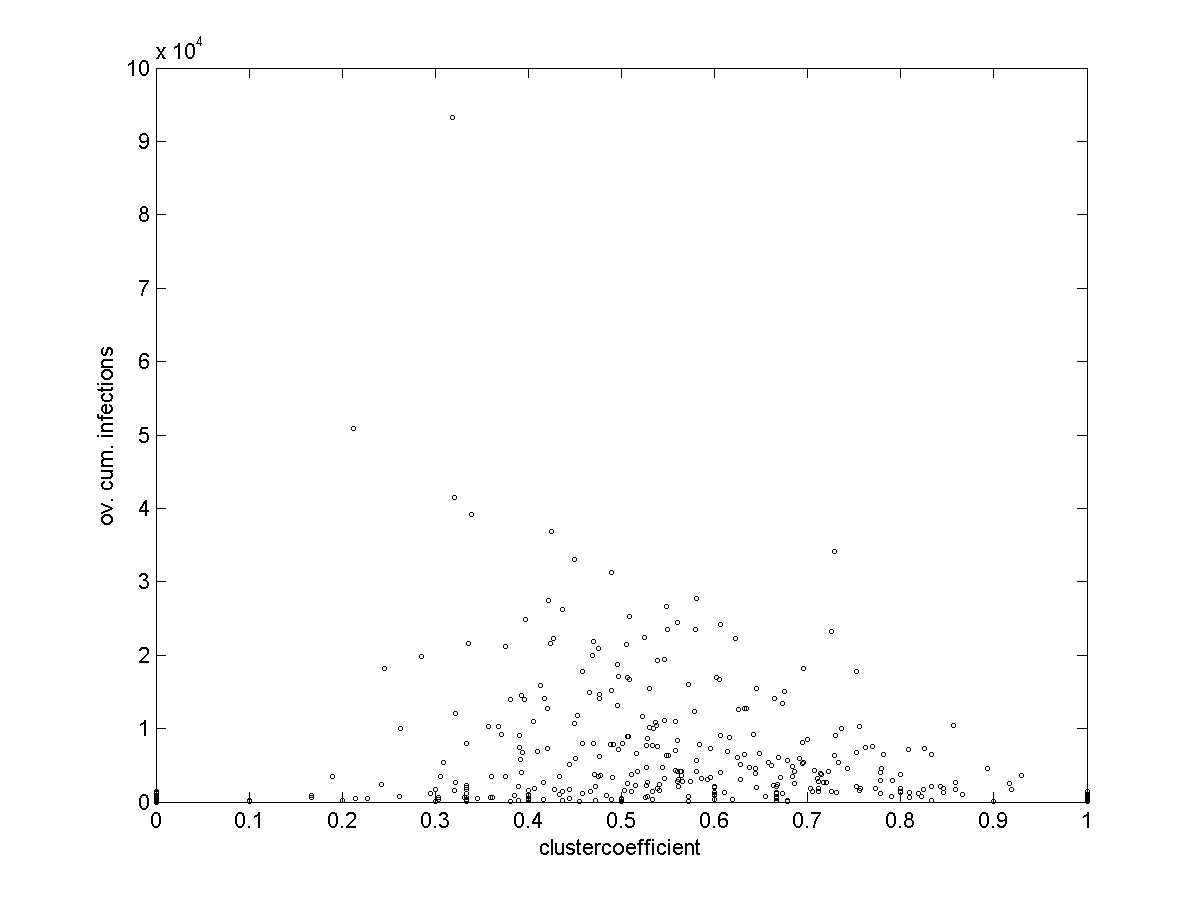
\includegraphics[width=6cm]{clustercVSov_cum_inf}
\end{figure}
\column{0.48\textwidth}
\begin{figure}
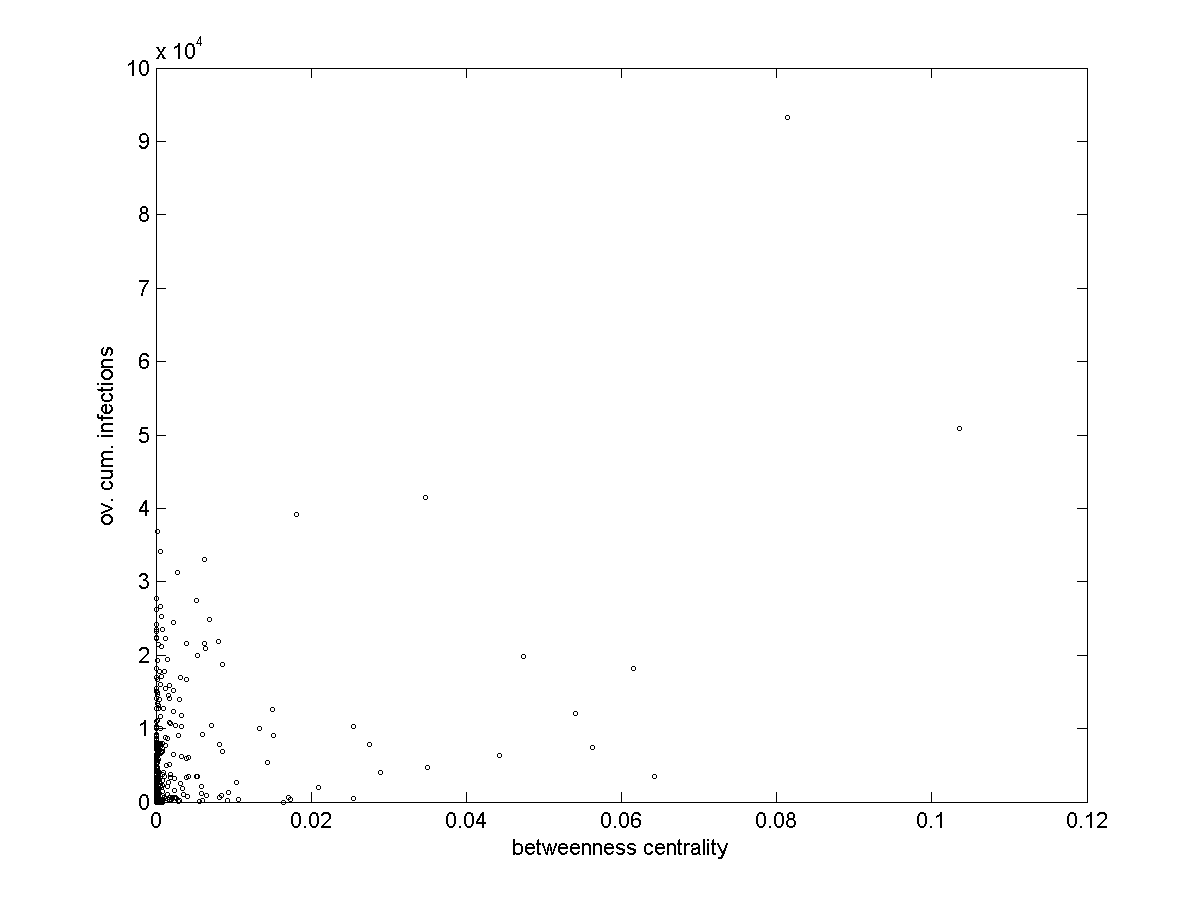
\includegraphics[width=6cm]{betwVSov_cum_inf}
\end{figure}
\end{columns}

\end{frame}


%------------------------------------------------
\section{Summary} % 
%------------------------------------------------

\begin{frame}
\frametitle{Summary}

\begin{itemize}

\item Under certain circumstances the population profiles of the agent-based model differs significantly from those of the homogeneous model.

\vspace{1cm}
\item Individuals being more important for information spreading, in terms of cumulative infections, were found. The betweenness centrality might be used to roughly predict those especially influential individuals.


\end{itemize}

\end{frame}


%------------------------------------------------

\begin{frame}
\Huge{\centerline{The End}}
\end{frame}

%----------------------------------------------------------------------------------------

\end{document} 

%------------------------------------------------

%\begin{frame}
%\frametitle{Multiple Columns}
%\begin{columns}[c] % The "c" option specifies centered vertical alignment while the "t" option is used for top vertical alignment

%\column{.45\textwidth} % Left column and width
%\textbf{Heading}
%\begin{enumerate}
%\item Statement
%\item Explanation
%\item Example
%\end{enumerate}

%\column{.5\textwidth} % Right column and width
%Lorem ipsum dolor sit amet, consectetur adipiscing elit. Integer lectus nisl, ultricies in feugiat rutrum, porttitor sit amet augue. Aliquam ut tortor mauris. Sed volutpat ante purus, quis accumsan dolor.

%\end{columns}
%\end{frame}

%------------------------------------------------

%\begin{frame}
%\frametitle{Table}
%\begin{table}
%\begin{tabular}{l l l}
%\toprule
%\textbf{Treatments} & \textbf{Response 1} & \textbf{Response 2}\\
%\midrule
%Treatment 1 & 0.0003262 & 0.562 \\
%Treatment 2 & 0.0015681 & 0.910 \\
%Treatment 3 & 0.0009271 & 0.296 \\
%\bottomrule
%\end{tabular}
%\caption{Table caption}
%\end{table}
%\end{frame}

%------------------------------------------------

%\begin{frame}
%\frametitle{Theorem}
%\begin{theorem}[Mass--energy equivalence]
%$E = mc^2$
%\end{theorem}
%\end{frame}

%------------------------------------------------

%\begin{frame}[fragile] % Need to use the fragile option when verbatim is used in the slide
%\frametitle{Verbatim}
%\begin{example}[Theorem Slide Code]
%\begin{verbatim}
%\begin{frame}
%\frametitle{Theorem}
%\begin{theorem}[Mass--energy equivalence]
%$E = mc^2$
%\end{theorem}
%\end{frame}\end{verbatim}
%\end{example}
%\end{frame}

%------------------------------------------------

%\begin{frame}
%\frametitle{Figure}
%Uncomment the code on this slide to include your own image from the same directory as the template .TeX file.
%\begin{figure}
%\includegraphics[width=0.8\linewidth]{test}
%\end{figure}
%\end{frame}

%------------------------------------------------

%\begin{frame}[fragile] % Need to use the fragile option when verbatim is used in the slide
%\frametitle{Citation}
%An example of the \verb|\cite| command to cite within the presentation:\\~

%This statement requires citation \cite{p1}.
%\end{frame}

%------------------------------------------------

%\begin{frame}
%\frametitle{References}
%\footnotesize{
%\begin{thebibliography}{99} % Beamer does not support BibTeX so references must be inserted manually as below
%\bibitem[Smith, 2012]{p1} John Smith (2012)
%\newblock Title of the publication
%\newblock \emph{Journal Name} 12(3), 45 -- 678.
%\end{thebibliography}
%}
%\end{frame}

